\documentclass[12pt,a4paper]{article}
\usepackage{blindtext}
\usepackage{graphicx}
\usepackage[utf8]{inputenc}
\usepackage[margin=0.65in]{geometry}
\usepackage{multicol}
\usepackage{wrapfig}
\usepackage[dvipsnames]{xcolor}
\usepackage{framed}
\usepackage[most]{tcolorbox}
\usepackage{pgfgantt}
\usepackage{tikz}
\usetikzlibrary{arrows.meta}
\usepackage[dvipsnames]{xcolor}
\definecolor{aliceblue}{rgb}{0.94, 0.97, 1.0}
\colorlet{shadecolor}{aliceblue}
\setlength\parindent{0pt}
\usepackage{charter}
\usepackage{environ}
\usepackage{tikz}
\usetikzlibrary{calc,matrix}
\usetikzlibrary{positioning,fit,calc}
\usepackage{float}
\usepackage{url}
% code by Andrew:
% http://tex.stackexchange.com/a/28452/13304
\makeatletter
\let\matamp=&
\catcode`\&=13
\makeatletter
\def&{\iftikz@is@matrix
	\pgfmatrixnextcell
	\else
	\matamp
	\fi}
\makeatother

\newcounter{lines}
\def\endlr{\stepcounter{lines}\\}

\title{COMPSCI 702 - Security for Smart-devices}
\date{Semester 1, 2018}
\begin{document}
\maketitle
\tableofcontents{}

\section*{Disclaimer}
\textit{This study guide is based off the lecture slides prepared for CS702. It is provided as-is and may contain errors, though effort has been made to minimize this. This resource is not exhaustive and may not contain additional content not covered by the slides.}
\newpage

\section{Access Control}
\subsection{Security objectives}
\begin{shaded}
\begin{itemize}
	\item \textbf{Confidentiality.} Protection of the data.
	\item \textbf{Integrity.} Ensure data is not altered by unauthorized parties.
	\item \textbf{Availability.} Ensure timely access to data.
	\item \textbf{Authentication.} Identify whether communicating entity is who it claims to be.
	\item \textbf{Authorization.} Regulate access to data.
\end{itemize}
\end{shaded}
\subsection{Access control requirements}
The inputs need to be \textit{reliable}, with authenticated entities or genuine information. The \textbf{principle of least privileges} grants the minimum set of access rights to do a job. Furthermore, only a special entity (administrator) can manage (grant/revoke/update) access rights.
\subsection{Elements of access control}
\begin{shaded}
\begin{itemize}
	\item \textbf{Subject.} An entity that can access objects. It can be a user or a process representing a user or an application.
	\item \textbf{Object.} An entity (file, directory, resource) that needs to be protected.
	\item \textbf{Access right.} An access right $r \in R$ describes how a subject $s \in S$ can access an object $o \in O$. Examples include: read, write, execute, create, delete, search, etc.
	\item \textbf{Access control function $f(s, o, r)$} looks up the access right $r$ for combination $(s, o)$. It grants access on a successful match.
	\item \textbf{Security administrator.} Entity that manages access rights.
	\item \textbf{Auditor.} Entity that inspects whole authorization system.
\end{itemize}	
\end{shaded}
\subsection{Access control models}
There are 5 main models for access control:
\begin{itemize}
	\item Discretionary access control (DAC),
	\item Mandatory access control (MAC),
	\item Role-based access control (RBAC),
	\item Usage control (UCON), and
	\item Policy-based access control (PBAC).
\end{itemize}
\subsubsection{Discretionary access control}
Users can protect what they own. The owner can grant access to subjects. Access is granted based on the identity of the requester. These mechanisms are adequate for honest users, but are vulnerable to Trojan horses.\\

DAC is used in operating systems and DBMS. An example is Linux file permissions: \texttt{rwxr-x--x}.

\subsubsection*{Access control matrix}
\begin{shaded}
\begin{center}
\begin{tabular}{lllll}
                            & File 1                                                                            & File 2                                                                            & File 3                                                                            & File 4                                                                          \\ \cline{2-5} 
\multicolumn{1}{l|}{User A} & \multicolumn{1}{l|}{\begin{tabular}[c]{@{}l@{}}owner\\ read\\ write\end{tabular}} & \multicolumn{1}{l|}{}                                                             & \multicolumn{1}{l|}{\begin{tabular}[c]{@{}l@{}}owner\\ read\\ write\end{tabular}} & \multicolumn{1}{l|}{}                                                           \\ \cline{2-5} 
\multicolumn{1}{l|}{User B} & \multicolumn{1}{l|}{read}                                                         & \multicolumn{1}{l|}{\begin{tabular}[c]{@{}l@{}}owner\\ read\\ write\end{tabular}} & \multicolumn{1}{l|}{write}                                                        & \multicolumn{1}{l|}{read}                                                       \\ \cline{2-5} 
\multicolumn{1}{l|}{User C} & \multicolumn{1}{l|}{\begin{tabular}[c]{@{}l@{}}read\\ write\end{tabular}}         & \multicolumn{1}{l|}{read}                                                         & \multicolumn{1}{l|}{}                                                             & \multicolumn{1}{l|}{\begin{tabular}[c]{@{}l@{}}own\\ read\\ write\end{tabular}} \\ \cline{2-5} 
\end{tabular}
\end{center}
An \textbf{access control list}	is a list of access rights on an object. A \textbf{capability list} refers to a user's permissions on different objects. In the diagram, columns are ACLs and rows are capability lists.
\end{shaded}
\subsubsection{Mandatory access control}
MAC restricts access on the basis of security labels. Entities cannot enable other entities to access their resources. Users have security clearance, and resources have security labels that contain data classification.\\

This model is used when information classification and confidentiality are very important, such as in the military. The \textbf{Bell-LaPadula model} (BLP) is used in the US Department of Defence. The \textbf{Biba model} is implemented in the FreeBSD MAC policy. A combined version is used in Android.

\subsubsection*{Bell-LaPadula model}
Goal: Control \textbf{confidentiality of information}.
\begin{itemize}
	\item \textbf{Simple security property.} No read up.
	\item \textbf{*(Star)property.} No write down.
	\item \textbf{Strong *(star)property} No write down and no write up.
\end{itemize}

\subsubsection*{Biba integrity model}
Goal: Control \textbf{integrity of information}.
\begin{itemize}
	\item \textbf{Simple integrity axiom.} No read down.
	\item \textbf{*(Star)-integrity axiom.} No write up.
\end{itemize}
\subsubsection{Role-based access control}
RBAC maps roles to access rights. Supports complex access control. Reduces administrative errors. Flexible to move users or permissions in/out of roles. Least privilege; restrict access according to needs.

\subsubsection*{RBAC model}
\begin{shaded}
\begin{itemize}
	\item \textbf{User.} A human being. Usually. They are assigned roles (\textbf{user assignment, UA}).
	\item \textbf{Permissions.} Approval of a mode of access to some object. They represent what operations could be performed on objects.
	\item \textbf{Roles.} Job title. Roles are assigned permissions (\textbf{permission assignment, PA}).
	\item \textbf{Assignments.} User-role and role-permission.
	\item \textbf{Session.} Mapping between user and an activated subset of assigned roles.
	\item \textbf{Constraints.} Constraintsd are present on sessions, assignments, and roles.
\end{itemize}	
\end{shaded}

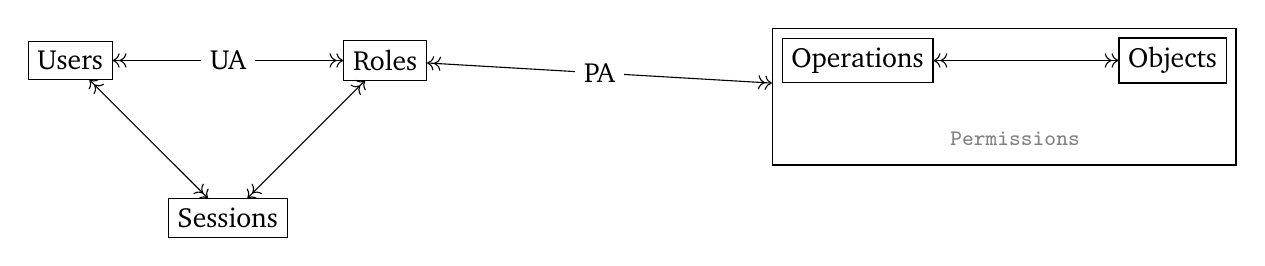
\begin{tikzpicture}[title/.style={font=\fontsize{8}{8}\color{black!50}\ttfamily}]
\node (h) at (12, 1) [title] {Permissions};
\node (a) at (0, 2) [rectangle, draw] {Users};
\node (b) at (4, 2) [rectangle, draw] {Roles};
\node (c) at (2, 0) [rectangle, draw] {Sessions};
\node (d) at (10, 2) [rectangle, draw] {Operations};
\node (e) at (14, 2) [rectangle, draw] {Objects};
\node (f) at (8, 2) [rectangle, draw, fit={(h) (d) (e)}] {};
\draw [<<->>] (a) -- (b) node [midway, fill=white] {UA};
\draw [<<->>] (a) -- (c);
\draw [<<->>] (b) -- (c);
\draw [<<->>] (b) -- (f) node [midway, fill=white] {PA};
\draw [<<->>] (d) -- (e);
\end{tikzpicture}

\subsubsection*{Controlling usage of resources}
DAC, MAC, and RBAC are concerned with checking access rights of entities. Once the access is granted, no more control is enforced.

\subsubsection{Usage control}
UCON doesn't just regulate access to an object, but also focuses on controlling usage. Addresses DRM. DAC, MAC, and RBAC can be expressed by UCON.

\subsubsection*{UCON model}
\begin{shaded}
\begin{itemize}
	\item \textbf{Subjects.} Entities that perform actions.
	\item \textbf{Objects.} Entities accessed by subjects.
	\item \textbf{Rights.} Set of actions.
	\item \textbf{Authorization.} Functional predicates that have to be evaluated for usage decision.
	\item \textbf{Obligations.} Functional predicates that verify mandatory requirements that must have been performed by subject.
	\item \textbf{Conditions.} Environmental/system based decision factors (time, status, etc.)
\end{itemize}	
\end{shaded}
\subsubsection{Policy-based access control}
In PBAC, an authorization policy governs access rights of subjects over objects. Policies are specified independently of entities. This provides a coherent view of access control in a system, and a separation between AC logic and enforcement mechanism.\\

An approach is XACML.

\subsubsection*{PBAC entities}
\begin{itemize}
	\item \textbf{Policy administrator.} Administrates access policies.
	\item \textbf{Policy administration point (PAP).} Interface for policy administration.
	\item \textbf{Policy store.} Repository to store policies.
	\item \textbf{Subject.} Entity that makes access requests.
	\item \textbf{Resources.} Target objects requested by subject.
	\item \textbf{Policy enforcement point (PEP).} Enforces access policies and grants access to resources.
	\item \textbf{Policy decision point (PDP).} Evaluates access policies.
	\item \textbf{Policy information point (PIP).} Provides contextual information.
\end{itemize}
\section{Android Security}
\subsection{Introduction to Android}
Android is a smartphone (open-source) OS currently developed by Google based on the Linux kernel. The SDK was released in November 2007 for Java, followed by the NDK (native development kit) in June 2009 for C and C++. The \textbf{Open Handset Alliance} is a consortium of 84 firms for developing open standards for mobile devices.\\

Android \textbf{fragmentation} is a problem. Vendors can customize the OS for their own devices by including their own apps. Some of these apps may compromise security/privacy as they have technical vulnerabilities. Vendors also might not push updates as frequently, and leave devices a few versions behind. Some vendors stop supporting their devices afterwards as well. \textit{The lack of support can lead to vulnerabilities.}\\

Android is considered \textbf{middleware} between the Linux kernel and its set of APIs. Android apps are mainly written in Java, and only Android apps can run on Android devices. Through the APIs, apps can access device information/components.

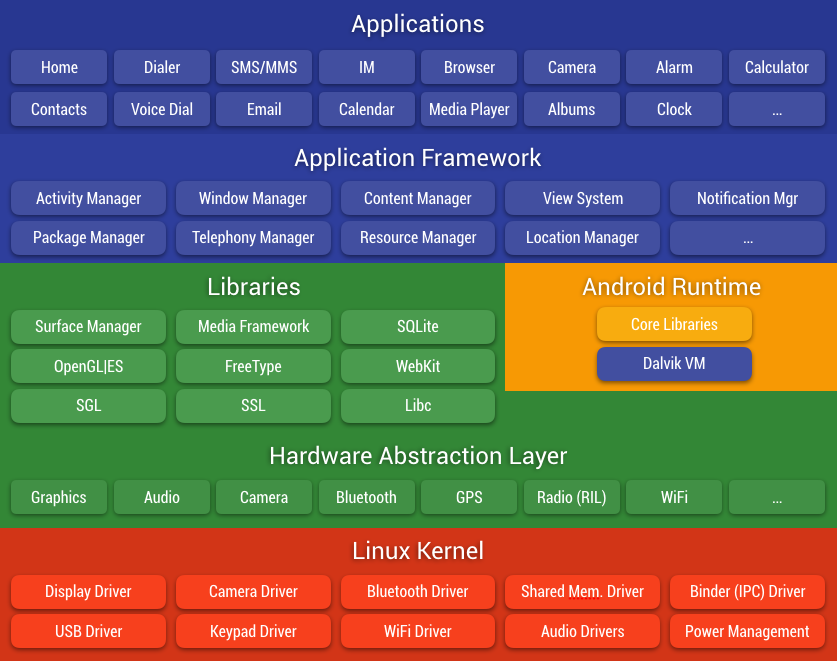
\includegraphics[width=\textwidth]{graphics/androidanatomy}

\paragraph{Linux kernel}
Android is built on the Linux kernel\footnote{It is \textbf{not} Linux.}. There is no \texttt{glibc} support, nor does it include the full set of Linux utilities. There are some kernel enhancements.\\

The Linux kernel was chosen as it has great memory/process management. It also has a permissions-based security model, a proven driver model, support for shared libraries. The Linux kernel is also open-source.

\paragraph{Binder}
Applications and services may run in separate processes but must communicate and share data. \textbf{Issue:} Inter-process communication (IPC) can introduce significant processing overhead and security holes. \textbf{Solution:} Driver to facilitate IPC.

\paragraph{Power management}
Mobile devices run on battery power with limited capacity. The power management features are built on top of Linux power management, but has more aggressive power management policy.

\subsubsection*{Native libraries}
Bionic \texttt{libc} is a custom \texttt{libc} implementation.\\

Why Bionic? \texttt{glibc} is licensed under LGPL, which prevents static linking of proprietary software. The size needs to be small as it will load in each process, and needs to be efficiency due to limited CPU power. \textbf{Bionic \texttt{libc}} is under the BSD license, is small, and efficient due to a custom pthread implementation. It does not support some POSIX features, is not compatible with \texttt{glibc}, and all native code must be compiled against Bionic.

\subsubsection*{Hardware abstraction layer}
This layer is a user-space C/C++ layer which separates the Android platform logic from the hardware interface.\\

A user-space HAL is necessary as 1) not all components have standardized kernel driver interfaces; 2) kernel drivers are licensed under GPL, which exposes any proprietary IP; and 3) Android has specific requirements for hardware drivers.

\subsubsection*{Android runtime}
\paragraph{Dalvik VM}
Android's custom clean room implementation. Provides application portability and runtime consistency. This runs Dalvik bytecode (optimized file format \texttt{.dex}). Java \texttt{.class}/\texttt{.jar} files are converted to \texttt{.dex} at build time.\\

The VM is also designed for embedded environment. It supports multiple virtual machine processes per device. It has a highly CPU-optimized bytecode interpreter, and uses runtime memory very efficiently.

\paragraph{Core libraries}
These are Core APIs for Java which provide a powerful and simple/familiar development platform. They are basically Java wrappers around C/C++ based libraries.

\subsubsection*{Application framework}
These are services essential for Android. Apps don't access them directly.

\subsubsection*{Applications}
These are applications.

\subsubsection{Runtime}
At startup, the bootloader loads the Linux kernel and starts the \texttt{init} process. The \texttt{init} process starts the \textbf{zygote} process, a nascent process that initializes a Dalvik VM instance. It forks on request to create VM instances for managed processes. It uses copy-on-write to maximize re-use and minimize footprint. \textit{There is an instance of DalvikVM per APK.}\\

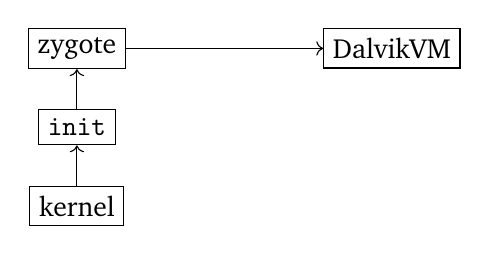
\begin{tikzpicture}[title/.style={font=\fontsize{8}{8}\color{black!50}\ttfamily}]
\node (a) at (0, 0) [rectangle, draw] {kernel};
\node (b) at (0, 1) [rectangle, draw] {\texttt{init}};
\node (c) at (0, 2) [rectangle, draw] {zygote};
\node (d) at (4, 2) [rectangle, draw] {DalvikVM};

\draw [->] (a) -- (b) node [midway] {};
\draw [->] (b) -- (c) node [midway] {};
\draw [->] (c) -- (d) node [midway] {};

\end{tikzpicture}

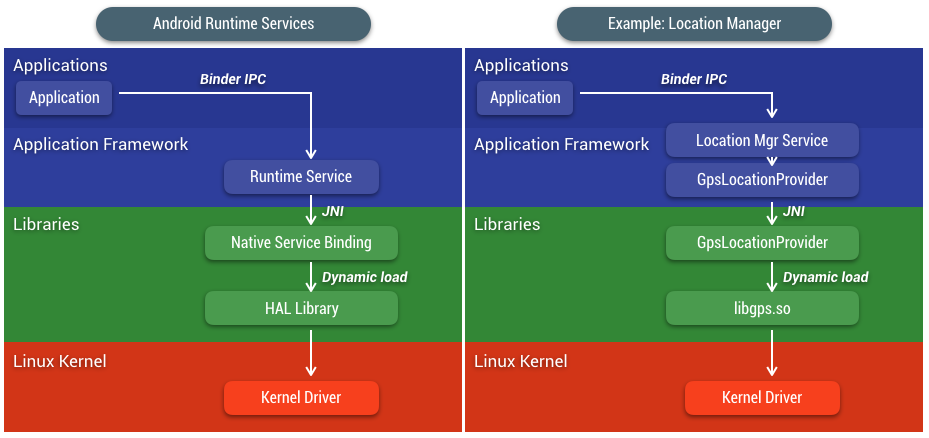
\includegraphics[width=\textwidth]{graphics/androidrt}

\subsubsection*{Android security objectives}
The goals are to protect user data, protect system resources (+network), and provide application isolation. 

\begin{shaded}
\textbf{Key Android security features:}
\begin{itemize}
	\item Robust security at OS level through Linux kernel
	\item Mandatory app sandboxing for all applications
	\item Secure IPC
	\item Application signing
	\item Application-defined and user-granted permissions
\end{itemize}	
\end{shaded}

\subsection{Android application model}
The Android application package (APK) consists of the following components:
\begin{itemize}
	\item \textbf{\texttt{classes.dex}.} Dalvik executable of Android app components
	\item \textbf{Resources and assets.} Images, string values, raw data, layouts, etc.
	\item \textbf{Native code.} C/C++ shared libraries linked dynamically
	\item \textbf{META-INF.} Certificate and signature information
	\item \textbf{Application manifest.} XML file that declares app metadata/components (names, intent filters, permissions). Its main elements are package info, app info (icon, etc.), activity component, etc.
\end{itemize}

Android requires that all apps be digitally signed with a certificate. Android apps used self-signed certificates. This certificate is used to identify the developer of an app. Android follows the \textbf{same-origin policy}. Android uses the same signing key-pair to ensure that updates come from the same developer.\\

An Android app is a combination of loosely coupled components. Each component can offer multiple entry points.
\begin{itemize}
	\item Activity: user interface
	\item Service: background services
	\item Content provider: database
	\item Broadcast receiver: mailbox for broadcasted messages
\end{itemize}

\subsubsection*{Intents}
\textbf{Intents} are named events and represent the \textit{intent} to do something, such as launching an activity, starting service, or broadcasting a message. Its payload and attributes describe the intended action. It can be sent/received by an app.\\

An \textbf{explicit} intent sets the target component name, such as \texttt{com.example.app.MainActivity}.\\

An \textbf{implicit} intent provides information including action, data, and type. This is resolved at runtime by the package manager. The Android framework will find a suitable receiver for this intent. For example: \texttt{Action=intent.ACTION\_VIEW; Data=www.youtube.com} will open an app that can show YouTube, such as the YouTube app or the default web browser.

\subsubsection*{Activity}
\begin{wrapfigure}{r}{0.5\textwidth}
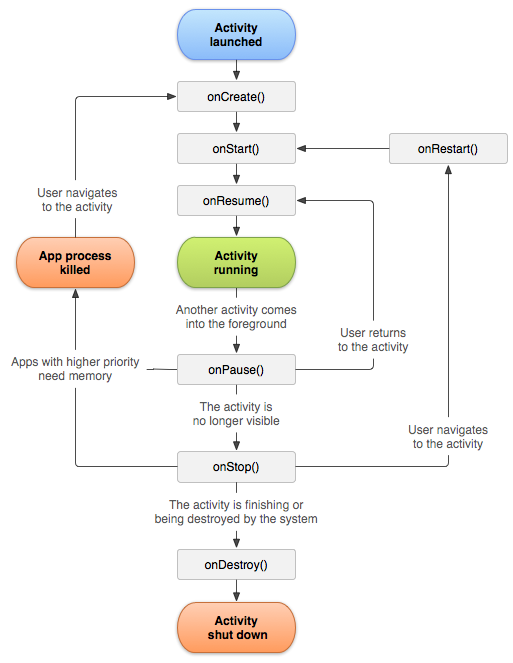
\includegraphics[width=0.5\textwidth]{graphics/activity_lifecycle}
\end{wrapfigure} 
An \textbf{activity} is a main building block of GUI applications. It is like a website; multiple activities represent multiple ``pages'', and the main activity is like the homepage. It is possible to move from an activity to another, just like navigating through pages.\\

There are system calls as state changes due to user actions. If there is another activity started, the on-going activity is paused. App process may be killed, and a stopped activity can be destroyed.\\

The \textbf{Activity Manager} is responsible for creating, destroying, and managing activities. When a user starts an application for the first time, the AM will create its activity and put it onto the screen. When the user switches screens, the AM will move the previous activity to a holding place, so if the user wants to go back to an older activity it can be started more quickly.\\

Older activities that haven't been used for a while will be destroyed to free space for current ones.

\subsubsection*{Service}
A \textbf{service} is a background process without a user interface, used to perform some long-running operation, such as downloading files or playing music. It can be local to the app or provided by other apps. Services can define a remote interface using the Android Interface Definition Language. The AIDL compiler creates skeleton for implementation of the service (stub). Services are started and stopped on demand.\\

App components start unbounded services. A \textbf{bounded service} acts as a server. The app component (client) logs in (binds) to the server, consumes the services, and then unbinds.\\

Use an \textbf{unbounded service} to do work if the app components don't need interaction with the service again. Use a \textbf{bounded service} if interaction is required.


\subsubsection*{Content providers}
\textbf{Content providers} are interfaces for sharing data between apps. The interfaces are simple: \texttt{select(), insert(), update(),} and \texttt{delete()}. They must be declared in the manifest with the \texttt{<provider>} tag.\\

Content providers are accessed by the URI \texttt{content://<authority>/<resource>}.\\

\paragraph{Contacts} Content provider that exposes user contact data to applications. The contacts app uses the contacts provider (a separate app) to retrieve contacts data. The contacts app does not have contacts data.

\paragraph{Settings} Exposes system settings to applications, including to Settings.

\paragraph{Media} Store responsible for storing/sharing media across applications.

\subsubsection*{Broadcast receiver}
A \textbf{broadcast receiver} is a component that responds to system-wide events. It's a mailbox for broadcast intent messages. Intent filters can be defined to indicate what messages to receive.\\

Events can come from the system (SMS, low battery), or an application (data update complete).\\

Broadcast receivers are Android's implementation of a system-wide publish/subscribe mechanism. The system or apps are publishers, and user apps are subscribers. A subscribing app can subscribe by indicating intent filters in the manifest or registering dynamically. The receiver will receive a triggered event if there is a subscription.\\

Events are broadcasted to a number of receivers who subscribe for the event.\\

A BR has to register with the Activity Manager and the Package Manager. This can be done through the manifest or programmatically\footnote{I highly doubt code details are examinable...}.
\begin{shaded}
\begin{lstlisting}
<receiver android:name=``MsgListener''>
   <intent-filter>
      <action android:name=``compsci702.intent.action.BROADCAST''/>
   </intent-filter>
</receiver>
\end{lstlisting}

The \texttt{MsgListener} class is responsible for processing the intent. The \texttt{<action>} tag specifies the intents to be received.\\

To do it programmatically, add an intent with \texttt{IntentFilter\#addAction()} and override \texttt{onReceive(Context c, Intent i)} for the action to be performed, then register the receiver and filter.

\end{shaded}
\begin{figure}[h]
\centering
\caption{Android build process}
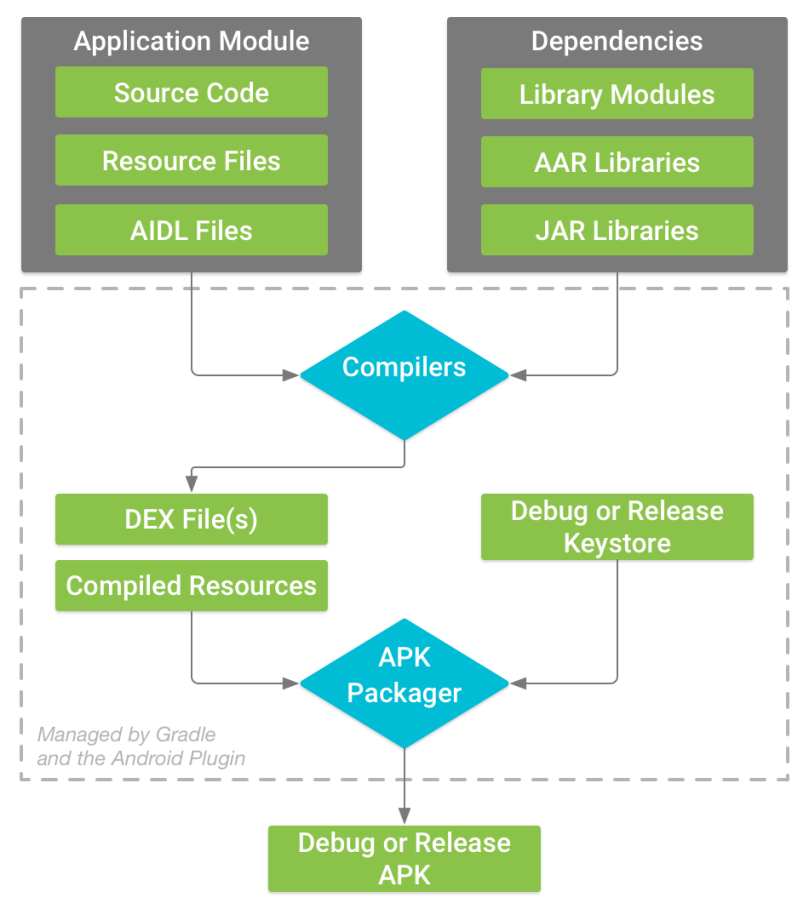
\includegraphics[width=0.5\textwidth]{graphics/build-apk}
\end{figure}

\subsection{Android ICC}
\subsubsection*{Android Binder}
Binder enables \textbf{inter-component communication} (ICC) in Android. It is implemented as a Linux kernel driver, as a customized version of Open Binder. It provides a simple RPC-like mechanism. Apps use Java methods to invoke ICC, then Android translates this into C++ invocations and system calls to the binder driver.\\

In Linux, processes communicate and share data through pipes, shared memory, and message queues. In Android, app components communicate through binder.\\


The \textbf{Activity Manager} is a service that apps use for ICC. It provides over 100 methods, including these common ones: \texttt{startActivity()}, \texttt{startBroadcast()}, \texttt{startService()}, and \texttt{bindService()}. Apps export services by publishing them through the Activity Manager.\\

The \textbf{Service Manager} is a special system service to keep track of available services. An app that wants to provide a service to others can publish its service through the Service Manager. Communication to the Service manager takes place through the Binder.\\

The Service Manager accepts these commands:
\begin{itemize}
	\item \textbf{Publish.} Used to publish a service within the Service Manager. Takes arguments: service name and address.
	\item \textbf{Get/check.} Returns an address of the service in form of handler. Takes argument: service name.
	\item \textbf{List.} Lists the service names registered with the Service Manager.
\end{itemize}

The Android middleware contains a \textbf{reference monitor} that mediates the establishment of ICC. This is part of the Activity Manager.

\subsubsection*{MAC security enforcement}
A reference monitor enforces MAC for regulating access to app components. Access to each component is restricted by assigning it an access permission label. Applications are assigned collections of permission labels. When a component initiates ICC, the reference monitor checks if its permission label is same as the target component's access permission label.\\

The Android middleware implements a reference monitor providing MAC enforcement about how apps access components.

\begin{figure}[h!]
\centering
\caption{A's ability to access B and C is determined by comparing the access permission labels on B and C with the collection of labels assigned to App 1.}
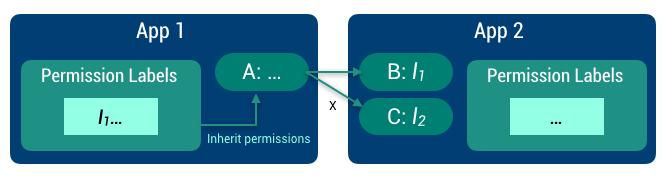
\includegraphics[width=0.9\textwidth]{graphics/plabels}
\end{figure}

Assigning permission labels to an app specifies its protection domain. Android's policy enforcement is mandatory: permission labels can't be changed until the app is reinstalled. This model restricts access to components and doesn't provide information flow guarantees.

\subsection{Sandboxing}
\textbf{Sandboxing} specifies which system resources an application is allowed to access. This limits malicious apps to perform actions only in the sandboxed environment. \\

There are two levels of sandboxing:
\begin{itemize}
	\item \textbf{Process level.} Each application is run in a dedicated process and access to sensitive resources depends on permissions. \begin{itemize} 
	\item Android assigns a unique User ID (UID) to each Android app.
	\item A UID (AppID) is generated at install time.
	\item It runs each app as a separate process with its UID.
	\item Apps run within the sandboxing environment in the kernel.
	\end{itemize}
	\item \textbf{Filesystem level.} Each application has its own private data directory and only the application can access its own data directory. \begin{itemize} 
	\item Each app is assigned a dedicated data directory.
	\item This applies to all apps (even native apps).
	\item Only the app has permission to read/write to its data directory.
	\end{itemize}
\end{itemize}

The app data directory is implemented based on Linux DAC. Permissions are set by the system \texttt{rwxrwxrwx}. Only the owner/root can change permissions.\\

System daemons and apps run under well-defined/constant UIDs. The root has UID 0. System UIDs are statically defined in the \texttt{android\_filesystem\_config.h} header file.\\

UIDs for system services start from 1000:
\begin{itemize}
	\item \texttt{android.uid.phone} (PHONE\_UID, 1001)
	\item \texttt{android.uid.bluetooth} (BLUETOOTH\_UID, 1002)
	\item \texttt{android.uid.log} (LOG\_UID, 1007)
	\item \texttt{android.uid.nfc} (NFC\_UID, 1027)
\end{itemize}

Apps can be installed using the same UID. Apps can share files and run in the same process. Shared UIDs are used by system apps which use the same set of resources. (Example: in Android 4.4, the system UI and keyguard share the same UID).\\

Shared UIDs aren't recommended for non-system apps, but is still available as long as the apps are signed with the same signing key.

\subsection{Permissions}
Apps are sandboxed, so they can only access their own files. Android can grant additional access rights (permissions) to apps. This helps Android control access to resources.\\

Apps request permissions defined in \texttt{AndroidManifest.xml}. Apps can request a set of additional permissions granted at runtime. A user may be asked to grant requested permissions. Android comes with a built-in list of pre-defined permissions. When new features come out, associated permissions are added as well. \textbf{Custom permissions} can be defined by system and user-installed apps.\\

An app that wants to receive incoming SMS (\texttt{RECEIVE\_SMS}) has to declare:

\begin{lstlisting}
<uses-permission android:name="android.permission.RECEIVE_SMS"/>
\end{lstlisting}

\subsubsection*{Permission management}
Permissions are assigned to each app by the package manager, which maintains a central database of installed packages with info about install path, version, certificate info, assigned permissions to each package, and a list of all permissions defined on a device. This database is in \texttt{/data/system/package.xml} and is updated every time an app is installed, updated, or uninstalled.

\subsubsection*{Permission protection levels}
The levels characterize potential risk in the permission and indicate the procedure that the system should follow when determining whether to grant the permission.

\begin{itemize}
	\item \textbf{Normal.} This is not security critical and is granted without asking users. \begin{itemize} \item\texttt{ACCESS\_NETWORK\_STATE} allows apps to access network information.\end{itemize}
	\item \textbf{Dangerous.} Grants access to user data or some control over the device. Involves functionalities that can cost money, so requires user approval. \begin{itemize}
	\item \texttt{READ\_SMS} allows apps to read SMS.
	\item \texttt{CAMERA} gives apps access to camera.
	 \end{itemize}
	 \item \textbf{Signature.} Only granted to requested apps that are signed with the same key as the app that declared the permission. Strongest permission level as it requires cryptographic key possession. Apps using these permissions are controlled by the same developer. Decided by system without requiring user intervention. Typically used by system apps that do device management.
	\begin{itemize}	 \item \texttt{NET\_ADMIN} allows configuration of network interfaces, IPSec, etc.
	\end{itemize}
	\item \textbf{SignatureOrSystem.} Granted to apps part of the system image or signed with the same key as the app that declared permission. Allows vendors to have pre-installed apps to share specific features that require a permission without having to share signing keys. Until Android 4.3, any app installed in the system partition was granted this permission. Since Android 4.4, apps need to be installed in \texttt{system/priv-app} to get this.
\end{itemize}

\textit{TODO: The diagrams on these slides...}

\section{iOS Security}
\section{Seminars}




\end{document}
